\documentclass[11pt,a4paper]{article}

%include polycode.fmt

\usepackage[margin=2.5cm]{geometry}
\usepackage{todonotes}
\usepackage{microtype}
\usepackage{amssymb,amsmath}
\usepackage{mathpazo}
\usepackage{accents}
\usepackage{longtable,booktabs}
\usepackage{dcolumn}
\usepackage{pgf}
\usetikzlibrary{shapes.geometric}
\usetikzlibrary{matrix}
\usepackage{natbib}
\usepackage{hyperref}
\usepackage[capitalise,noabbrev,nameinlink]{cleveref}
\hypersetup{
  pdftitle={Pipelining in Ouroboros chain diffusion},
  pdfborder={0 0 0},
  breaklinks=true
}

\DeclareMathOperator{\dom}{dom}
\newcommand\restrict[2]{\left.#1\right||_{#2}}
\newcommand\deltavar[1]{\accentset{\Delta}{#1}}

\begin{document}

\title{Pipelining in Ouroboros chain diffusion\\
       {\large \sc An IOHK discussion paper}}
\date{Version 0.3, November 2021}
\author{Duncan Coutts      \\ {\small \texttt{duncan@well-typed.com}} \\
                              {\small \texttt{duncan.coutts@iohk.io}} \\
   \and Matthias Fitzi     \\ {\small \texttt{matthias.fitzi@iohk.io}}
   }

\maketitle

\section{Purpose}

The purpose of this document is to present a possible change to the algorithm
for Ouroboros chain diffusion that could allow for higher block validation times
for the same choice of the $\Delta$~diffusion time.

We will also attempt to analyse the algorithm, and review its implications and
what implementation changes would be necessary to make the change in practice.

\tableofcontents

\section{Acknowledgements}

The ideas presented here are inspired by and based on discussions with several
people from the research and engineering groups: Giorgos Panagiotakos,
Sandro Coretti-Drayton, Karl Knutsson, Marcin Szamotulski, Nick Frisby,
Neil Davies, Peter Thompson and Philipp Kant.

\section{Context}

While the research team have been considering the design for Ouroboros Leios
(using input endorsers) it has spawned some ideas for potential changes to
the existing Praos algorithm, which may also enable more even (and therefore
more efficient) use of network and CPU resources. In discussion with the
engineering network and consensus teams these ideas multiplied into a range of
plausible options.

In this document we will only present the \emph{least radical} of these options,
that we believe would involve fewest changes to the design or implementation,
but that nevertheless may provide a substantial benefit.

\section{Introduction}

The key idea is to forward block bodies \emph{before} having fully validated
them. This takes the block body validation time out of the critical path of
block diffusion. It allows the validation time on each `hop' in the path to be
overlapped with sending the block onto the next node in the path.

Supposing that there are typically $N$ hops in the path between block producers
within the network, and block body validation takes $V$ seconds, then in
principle then change could save $(N-1) V$ seconds in the overall diffusion
time. Equivalently, instead of having to fit $N$ validations into the $\Delta$
time budget, we need only fit $1$. This makes more efficient use of the
$\Delta$ time budget, which could be used to increase block sizes and/or
increase the block validation time (such as longer running scripts).

\section{The existing block relaying scheme}

The main steps on each node on the critical path of block relaying is roughly
as follows
\begin{enumerate}
\item transmit the block header (from upstream peer);
\item validate the block header;
\item request and transmit the block body (from upstream peer);
\item validate the block body and extend the local chain;
\item transmit the block header (to downstream peers);
\item transmit the block body (to downstream peers);
\end{enumerate}
On a stylised time line (with time running from left to right), we can depict
this as
\begin{center}
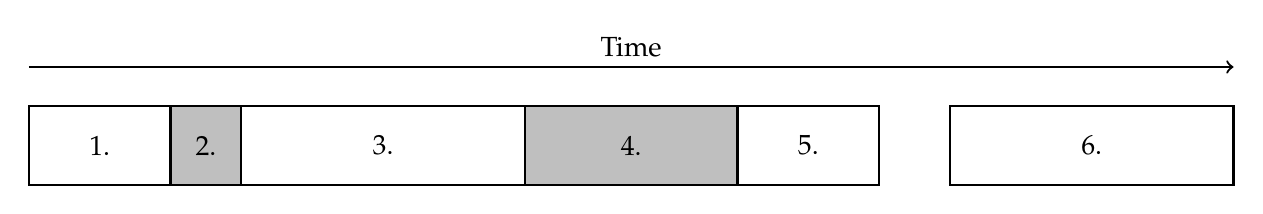
\begin{tikzpicture}
\begin{scope}[thick, xscale=0.9]

\draw (0,0) rectangle (2,1);
\draw[fill=lightgray] (2,0) rectangle (3,1);
\draw (3,0) rectangle (7,1);
\draw[fill=lightgray] (7,0) rectangle (10,1);
\draw (10,0) rectangle (12,1);
\draw (13,0) rectangle (17,1);

\draw (1,  0.5) node {1.};
\draw (2.5,0.5) node {2.};
\draw (5,  0.5) node {3.};
\draw (8.5,0.5) node {4.};
\draw (11, 0.5) node {5.};
\draw (15, 0.5) node {6.};

\draw[->] (0, 1.5) -- (17, 1.5);
\draw     (8.5, 1.5) node[anchor=south] {Time};

\end{scope}
\end{tikzpicture}
\end{center}
Of course this is one hop in the relaying and in a network there will typically
be 5 -- 7 such hops between the current block producer, and the other
block producers. In the current design we fully validate blocks before relaying
them, so the overall timeline looks like this

\begin{center}
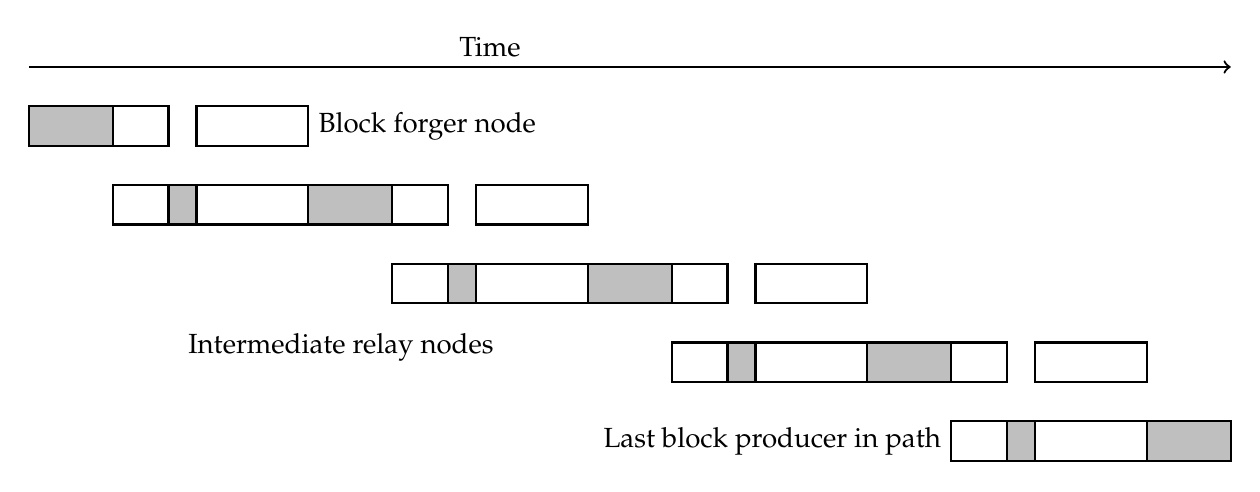
\begin{tikzpicture}
\begin{scope}[thick, xscale=0.355, yscale=0.5]

\begin{scope}
  \draw[fill=lightgray] (7,0) rectangle (10,1);
  \draw (10,0) rectangle (12,1);
  \draw (13,0) rectangle (17,1);
  \draw (17, 0.5) node[anchor=west] {Block forger node};
\end{scope}

\begin{scope}[xshift=10cm, yshift=-2cm]
  \draw (0,0) rectangle (2,1);
  \draw[fill=lightgray] (2,0) rectangle (3,1);
  \draw (3,0) rectangle (7,1);
  \draw[fill=lightgray] (7,0) rectangle (10,1);
  \draw (10,0) rectangle (12,1);
  \draw (13,0) rectangle (17,1);
\end{scope}

\begin{scope}[xshift=20cm, yshift=-4cm]
  \draw (0,0) rectangle (2,1);
  \draw[fill=lightgray] (2,0) rectangle (3,1);
  \draw (3,0) rectangle (7,1);
  \draw[fill=lightgray] (7,0) rectangle (10,1);
  \draw (10,0) rectangle (12,1);
  \draw (13,0) rectangle (17,1);
  \draw (4, -0.5) node[anchor=north east] {Intermediate relay nodes};
\end{scope}

\begin{scope}[xshift=30cm, yshift=-6cm]
  \draw (0,0) rectangle (2,1);
  \draw[fill=lightgray] (2,0) rectangle (3,1);
  \draw (3,0) rectangle (7,1);
  \draw[fill=lightgray] (7,0) rectangle (10,1);
  \draw (10,0) rectangle (12,1);
  \draw (13,0) rectangle (17,1);
\end{scope}

\begin{scope}[xshift=40cm, yshift=-8cm]
  \draw (0,0) rectangle (2,1);
  \draw[fill=lightgray] (2,0) rectangle (3,1);
  \draw (3,0) rectangle (7,1);
  \draw[fill=lightgray] (7,0) rectangle (10,1);
  \draw (0, 0.5) node[anchor=east] {Last block producer in path};
\end{scope}

\draw[->] (7, 2) -- (50, 2);
\draw     (23.5, 2) node[anchor=south] {Time};

\end{scope}
\end{tikzpicture}
\end{center}


\section{The proposed block relaying scheme}

By changing forwarding the block as soon as it has arrived locally, the
validation time is overlapped with sending and the overall timeline becomes
quite a bit shorter.
\begin{center}
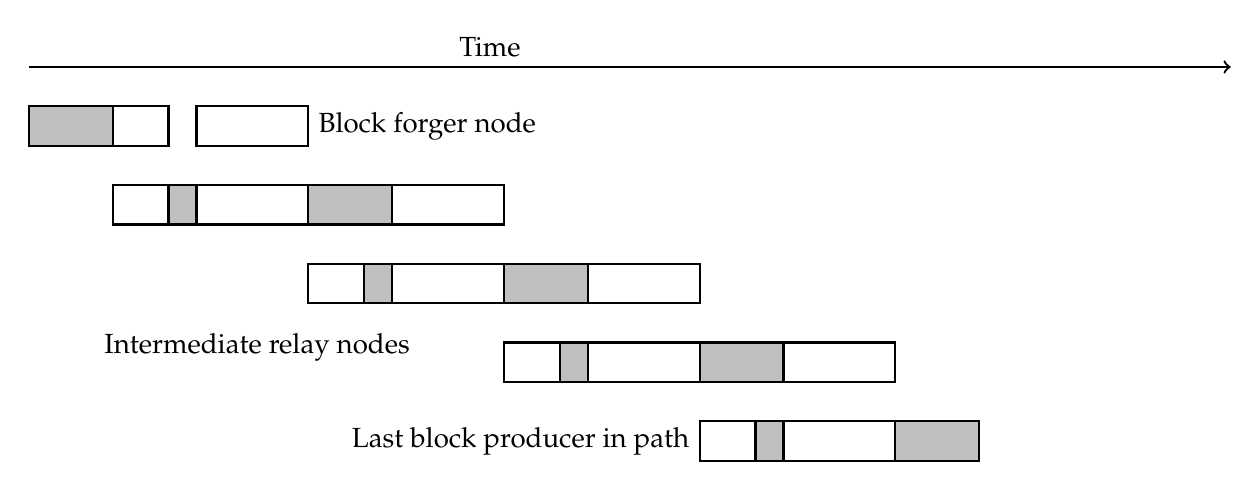
\begin{tikzpicture}
\begin{scope}[thick, xscale=0.355, yscale=0.5]

\begin{scope}
  \draw[fill=lightgray] (7,0) rectangle (10,1);
  \draw (10,0) rectangle (12,1);
  \draw (13,0) rectangle (17,1);
  \draw (17, 0.5) node[anchor=west] {Block forger node};
\end{scope}

\begin{scope}[xshift=10cm, yshift=-2cm]
  \draw (0,0) rectangle (2,1);
  \draw[fill=lightgray] (2,0) rectangle (3,1);
  \draw (3,0) rectangle (7,1);
  \draw[fill=lightgray] (7,0) rectangle (10,1);
  \draw (10,0) rectangle (14,1);
\end{scope}

\begin{scope}[xshift=17cm, yshift=-4cm]
  \draw (0,0) rectangle (2,1);
  \draw[fill=lightgray] (2,0) rectangle (3,1);
  \draw (3,0) rectangle (7,1);
  \draw[fill=lightgray] (7,0) rectangle (10,1);
  \draw (10,0) rectangle (14,1);
  \draw (4, -0.5) node[anchor=north east] {Intermediate relay nodes};
\end{scope}

\begin{scope}[xshift=24cm, yshift=-6cm]
  \draw (0,0) rectangle (2,1);
  \draw[fill=lightgray] (2,0) rectangle (3,1);
  \draw (3,0) rectangle (7,1);
  \draw[fill=lightgray] (7,0) rectangle (10,1);
  \draw (10,0) rectangle (14,1);
\end{scope}

\begin{scope}[xshift=31cm, yshift=-8cm]
  \draw (0,0) rectangle (2,1);
  \draw[fill=lightgray] (2,0) rectangle (3,1);
  \draw (3,0) rectangle (7,1);
  \draw[fill=lightgray] (7,0) rectangle (10,1);
  \draw (0, 0.5) node[anchor=east] {Last block producer in path};
\end{scope}

\draw[->] (7, 2) -- (50, 2);
\draw     (23.5, 2) node[anchor=south] {Time};

\end{scope}
\end{tikzpicture}
\end{center}

Alternatively, this saving can be used to substantially increase the block
validation time.
\begin{center}
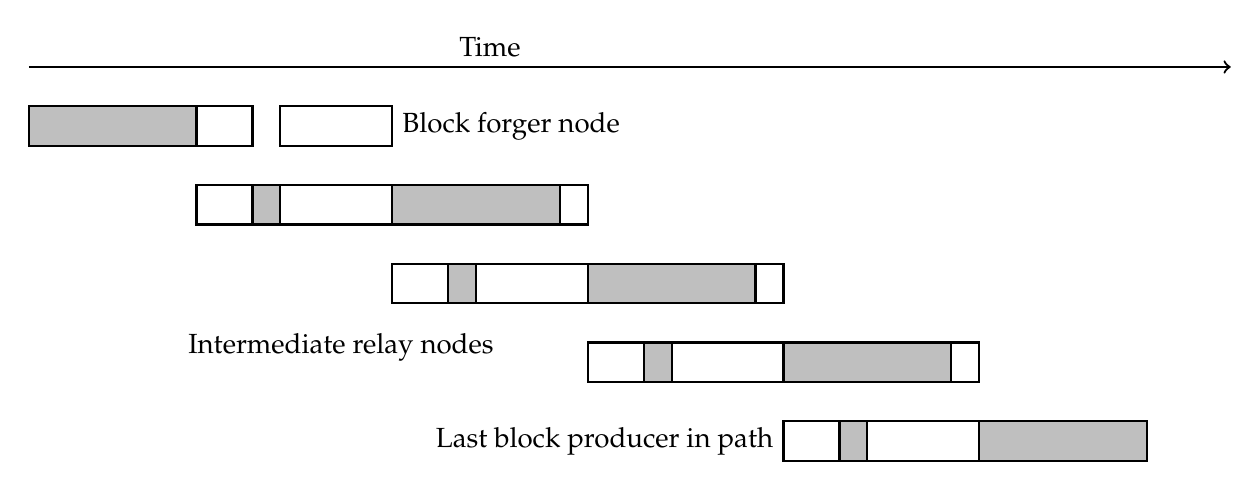
\begin{tikzpicture}
\begin{scope}[thick, xscale=0.355, yscale=0.5]

\begin{scope}
  \draw[fill=lightgray] (7,0) rectangle (13,1);
  \draw (13,0) rectangle (15,1);
  \draw (16,0) rectangle (20,1);
  \draw (20, 0.5) node[anchor=west] {Block forger node};
\end{scope}

\begin{scope}[xshift=13cm, yshift=-2cm]
  \draw (0,0) rectangle (2,1);
  \draw[fill=lightgray] (2,0) rectangle (3,1);
  \draw (3,0) rectangle (7,1);
  \draw[fill=lightgray] (7,0) rectangle (13,1);
  \draw (13,0) rectangle (14,1);
\end{scope}

\begin{scope}[xshift=20cm, yshift=-4cm]
  \draw (0,0) rectangle (2,1);
  \draw[fill=lightgray] (2,0) rectangle (3,1);
  \draw (3,0) rectangle (7,1);
  \draw[fill=lightgray] (7,0) rectangle (13,1);
  \draw (13,0) rectangle (14,1);
  \draw (4, -0.5) node[anchor=north east] {Intermediate relay nodes};
\end{scope}

\begin{scope}[xshift=27cm, yshift=-6cm]
  \draw (0,0) rectangle (2,1);
  \draw[fill=lightgray] (2,0) rectangle (3,1);
  \draw (3,0) rectangle (7,1);
  \draw[fill=lightgray] (7,0) rectangle (13,1);
  \draw (13,0) rectangle (14,1);
\end{scope}

\begin{scope}[xshift=34cm, yshift=-8cm]
  \draw (0,0) rectangle (2,1);
  \draw[fill=lightgray] (2,0) rectangle (3,1);
  \draw (3,0) rectangle (7,1);
  \draw[fill=lightgray] (7,0) rectangle (13,1);
  \draw (0, 0.5) node[anchor=east] {Last block producer in path};
\end{scope}

\draw[->] (7, 2) -- (50, 2);
\draw     (23.5, 2) node[anchor=south] {Time};

\end{scope}
\end{tikzpicture}
\end{center}
Before we analyse the risks it is important to be precise about which checks
we would still do promptly and which would be deferred. Checks that would still
be done:
\begin{enumerate}
\item all the header checks, including the KES and VRF;
\item the hash check that the block body content matches the header;
\item nodes relaying blocks would only relay a single block in advance of
      validating the block body; and
\item block producers would still validate the block body before creating a new
      block.
\end{enumerate}
The only check that would be deferred is that on the block body content.

\section{Analysis of DoS risks}

Of course the immediate concern is whether doing less prompt validation would
open any new opportunities for denial-of-service attacks. In general the reason
we take a very conservative approach to chain diffusion -- in which we validate
fully and promptly -- is to avoid denial-of-service attacks. The general
principle has been that while we have found ways to bound the amount of work
honest nodes need to do for valid block data, it is substantially harder to
bound if we propagate invalid data.

That said, the goal is not to prevent invalid data being relayed over the
network graph. The goal is to prevent honest nodes from being required to do an
unbounded amount of work, and indeed more stringently, to prevent honest nodes
from having to do more work than the dishonest nodes engaged in an attack. Thus
if we can relax or defer validation without increasing the work compared to the
normal valid case, then we may be ok. In particular we need to avoid any
situations where previously we did one expensive step and now we would do many.

The combination of checks 1.~and 2.~above should mean that the possibly-invalid
block is one that was signed by the block producer (KES check), who was
authorised to create a block in this slot (VRF check). This should mean that
there cannot be more of them in total than in the case of valid blocks. In
particular intermediate nodes cannot forge any extra or altered block without
falling foul of these checks. Thus it should be the case that only the
authorised block producer can create many valid blocks, or many valid block
headers with invalid block bodies.

\subsection{Many valid block headers}
\label{many-valid-block-headers}

As noted above, it is already possible for authorised block producers to sign
many valid blocks in their slot. It is instructive to see how we can avoid
honest nodes doing an unbounded amount of work in this situation.

Suppose one or more adversarial nodes are slot leaders (e.g. in recent slots)
and they extend the current chain with multiple different but \emph{valid}
blocks. They could each create multiple blocks individually, or collaborate to
extend each others' chains. Either way, the chains will differ only in the final
few blocks. Now suppose an honest node becomes aware of many of these different
chains (e.g. from different peers). The honest node will validate and adopt the
first one it manages to download (though it will try to pick the longest first).
The question now is whether the honest node will stop here or if it will be
persuaded to adopt a bounded or an unbounded number of the alternative chains.

Chains are ordered by the chain selection order. Chains will only be adopted if
they are strictly better in that ordering. The ordering is the lexicographic
combination of
\begin{enumerate}
\item order by chain length (longer chains preferred);
\item if last block slot numbers are the same then order by whether this node produced the block or not (locally produced blocks preferred);
\item if the last blocks were issued by the same entity (by SPO cold key) then order by the hot key certificate issue number (higher cert issue numbers preferred);
\item order by VRF value (lower VRF value preferred).
\end{enumerate}
An appropriate way to analyse this is to argue that there can only be bounded
progress in this order.
\begin{enumerate}
\item In the short term, the chain length is bounded by the Ouroboros leader
      schedule.
\item The second condition is only boolean, so is bounded.
\item The certificate counters are controlled by the block issuers and are not
      inherently bounded. This needs special treatment to establish a bound.
\item The VRF value depends on the identity of the block issuer, but its value
      is not under the issuer's control. We rely on the property of the VRF
      primitive that it's only possible to create a single valid value per
      block issuer per slot. Given this, the number of different VRF values is
      bounded by the number of different authorised block issuers (since the
      end of the most recent common chain) which is then bounded by the
      Ouroboros leader schedule.
\end{enumerate}
So the only case that needs special treatment is bounding the certificate issue
numbers.

The purpose of the certificate issue numbers is to allow a block producer to
cycle their hot keys and in particular to be able to issue a new hot key if the
current hot key becomes compromised. The reason to compare on certificate issue
numbers at all is for the situation where a compromised hot key is being used
to sign blocks. In this situation the true owner needs to issue a new hot key
with a new higher certificate issue number and use that to sign blocks. This
means the stolen key and the new key (with corresponding certs) may be being
used at the same time and they have to compete to be selected. This is why the
chain selection rule prefers the later issue number, so it will be selected
even if the block signed by the compromised key arrives first and is thus
selected first.

In principle the certificate issue numbers are not bounded, but the use case
of recovering from compromised keys does not require more than two issue
numbers. So `progress' in the certificate issue number can be bounded by
allowing at most two different blocks with the same issuer in the same slot.
There is also a `no regression' rule on the issue numbers used on the chain, so
even if an attacker has several compromised certificates, then as soon as they
use a later one then earlier ones can no longer be used again.

\subsection{Many valid block bodies}

The case for many block bodies is straightforward: they make no difference to
chain selection. So there being multiple different blocks with different
content does not alter the informal argument above. It is certainly adversarial
behaviour for a single block producer to create multiple different blocks in a
slot, but it does not directly create more work for honest nodes. A node that
has adopted one, will not select another from the same producer since it is not
better in the chain selection ordering.

\subsection{Many invalid block bodies}

If we postpone block body validation in the way proposed then all of the
considerations about many valid blocks still apply, and in addition we must
analyse the new cases for invalid block bodies. For this part of the analysis
we can presume that the block header is valid.

The bounding argument for the valid block case relies on making strict
progress in the chain selection ordering, and the overall opportunity to make
progress being bounded. The immediate difficulty in trying the same argument
with invalid block bodies is that once we discover they are invalid and we
stick to our current chain, then we have not made any progress in the chain
selection ordering. We are back in the same state where we are prepared to
consider fresh (or perhaps even the same) invalid blocks.

Under the full prompt validation model when we encounter an invalid block we
can promptly cut off all peers that gave us that invalid block (even peers
that just gave us the header). We cannot do that under the delayed block body
validation proposal because we can no longer pin the blame on the immediate
peer for failing to validate the block body before sending it to us.

Fortunately this problem does not appear insurmountable. We can still pin the
blame for a bad block on the issuer of the block. The block issuer is typically
not a direct peer so we cannot use disconnection as a remedy. If however we
use some state to temporarily remember the block issuer then we can use that to
simply not consider any more blocks signed by this issuer in this slot. They
have demonstrated themselves to be adversarial by signing a bad block and we
don't have to spend more resources considering any more blocks from them in
the short term. Note that for this purpose we must identify the block issuer
by the hot key certificate and not the `cold' permanent identity. This is
because a compromised hot key could be used to sign bad blocks, and that ought
still to be a situation a block producer can recover from by signing a new
certificate with a higher issue number.

It appears that it would be sufficient to remember bad block issuers
(identified by certificate) only until the current chain is sucessfully
extended. This would avoid considering more than a single bad block from any
recent issuer. The number of recent adversarial issuers (and thus the size of
the tracking set) is bounded by the leadership schedule and the honest stake
assumption. The certificate counters are bounded (or can be bounded) as
described in \cref{many-valid-block-headers}.

\section{Implementation changes}

The main change would be to introduce the notion of a `tentative chain'. This
is either the same as the current chain or is the current chain extended by a
single `tentative' block (header).

The tentative chain (of headers) would become the source for chain sync for
downstream peers, and the tentative block (including body) would also be
available for block fetch by downstream peers.

The tentative chain would be reset to be equal to the current chain every time
the current chain changes (i.e. is directly extended or switches to a longer
fork). It would also be reset if the tentative block is found to be invalid.

The tentative chain would be set with a tentative block whenever:
\begin{enumerate}
\item a new block is presented to the chain database which directly extends
      the current chain;
\item after the block is entered into the volatile db;
\item and the tentative chain is equal to the current chain.
\end{enumerate}
The first point ensures that this takes place after the block body content has
been checked against the header. The second ensures that the block will be
accessible to block fetch. The third point ensures that we do not keep changing
the tentative block. It's a one time change until the block validation catches
up and sets the current chain (or finds it to be invalid).

\end{document}
